\documentclass{article}
\usepackage[UTF8]{ctex}
\usepackage{float} %设置图片浮动位置的宏包
\usepackage{graphicx} %插入图片的宏包
\usepackage{subfigure} %插入多图时用子图显示的宏包
\usepackage{listings}
\usepackage{xcolor}
\usepackage{geometry}
\usepackage{amsmath}
\usepackage{multirow}
\newcommand{\upcite}[1]{\textsuperscript{\textsuperscript{\cite{#1}}}}

\geometry{
	a4paper,
	total={170mm,257mm},
	left=20mm,
	top=20mm,
}
\title{\vspace{-3cm} \textbf{基于知识图谱的推荐系统概述}}
\date{}

\begin{document}
	\maketitle
	
	\vspace{-2cm}
	
	\section{推荐系统背景}
	随着互联网时代的发展,数据爆炸带来的信息过载尤为显著。作为一种信息过滤系统\upcite{1},推荐系统已应用到电商、影视、旅游等各行各业。推荐系统能通过对大规模群体数据学习,实现用户群体特征匹配,从而帮助用户有效地从海量数据中识别出感兴趣的内容。 
	
	本文将从推荐系统展开,分别介绍传统的推荐系统和基于知识图谱的推荐系统,本文的思维框架图如图1所示:
	\begin{figure}[H]
	\centering
	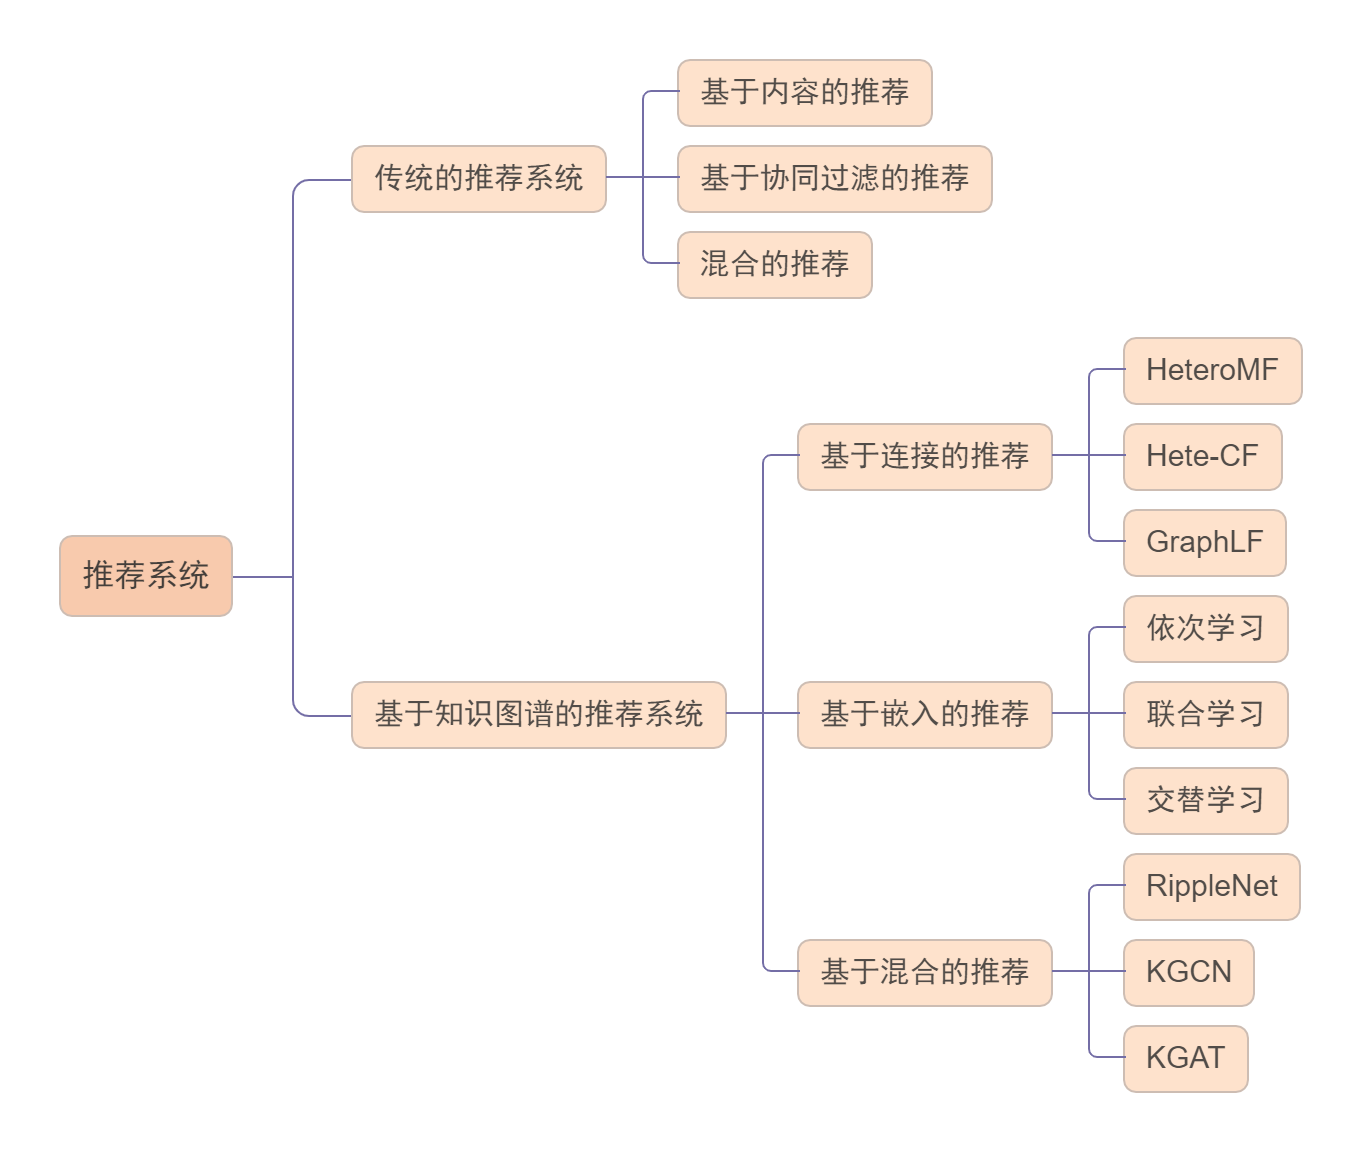
\includegraphics[width=8cm]{pt3.png}% 图片相对位置
	\vspace{-0.5cm}
	\caption{思维框架图} % 图片标题 
	\end{figure}
	
	\section{传统的推荐系统:以协同过滤为例}
	传统的推荐系统主要可分为基于内容的推荐、基于协同过滤的推荐和混合的推荐三种类型\upcite{1},其中,最经典和出名的当属协同过滤推荐算法。其总体可分为三个步骤:
	
	(1)构建评分矩阵。
	
	以通过用户对某一物品进行打分等方式收集用户的对物品的偏好,用户评分是算法的数据基础\upcite{2}。
	假设系统中有m个用户和n个物品,用$U$={$U_1$,$U_2$,...,$U_m$}表示用户集合,用$I$={$I_1$,$I_2$,...,$I_n$}表示物品集合,则用户${U_x}$对物品${I_y}$的评分为${S_{x,y}}$,用矩阵${R_{mxn}}$表示如式(1)所示:
	\begin{equation}
	R=\left(\begin{array}{ccc}
	S_{1,1} & \cdots & S_{1, n} \\
	\vdots & & \vdots \\
	S_{m, 1} & \cdots & S_{m, n}
	\end{array}\right)
	\end{equation}
	
	(2)计算物品相似度。
	物品向量的相似度可以用余弦相似度作为评价标准。将用户对某个物品的评分当成1个m维向量,则某个物品$I_i$的评分向量为$I_i=\{{S_{1,i},S_{2,i},...,S_{m,i}}\}$,物品$I_j$的评分向量为$I_j=\{{S_{1,j},S_{2,j},...,S_{m,j}}\}$,计算$I_i$与$I_j$的余弦相似度:
	\begin{equation}
	\operatorname{sim}_{\mathrm{s}}\left(I_{i}, I_{j}\right)=\cos \left(\boldsymbol{I}_{i}, \boldsymbol{I}_{j}\right)=\frac{\sum S_{u, i} \cdot S_{u, j}}{\sqrt{\sum S_{u, i}^{2}} \cdot \sqrt{\sum S_{u, j}^{2}}}
	\end{equation}
	余弦相似度在实际中未能考虑用户评分的差异。例如,有些用户给所有物品的评分普遍评分较高,有
	些用户则普遍给出较低分数。这样用户对于同样评分的物品的喜好实际上并不相同。因此,采用修正的余弦相似度,公式如下所示:
	\begin{equation}
	\operatorname{sim}_{c}\left(I_{i}, I_{j}\right)=\frac{\sum_{U_{i, j}}\left(S_{u, i}-\bar{S}_{u}\right) \cdot\left(S_{u, j}-\bar{S}_{u}\right)}{\sqrt{\sum_{U_{i}}\left(S_{u, i}-\bar{S}_{u}\right)^{2}} \cdot \sqrt{\sum_{U_{j}}\left(S_{u, j}-\bar{S}_{u}\right)^{2}}}
	\end{equation}
	
	其中,$\bar{S}_{u}$表示用户的平均评分。计算物品相似度时利用修正的余弦相似度会将用户对物品的评分减去用户历史评分的均值,从而避免了用户给出评分时评分标准不一致的问题。
	
	(3)近邻选择。
	
	近邻选择算法有K近邻选择和阈值法2种,其中K近邻选择算法是将相似度进行排序从而筛选出前K个最相似的物品进行推荐。阈值法是设置阈值T,将相似度高于阈值T的物品列入推荐列表。

	\section{基于知识图谱的推荐系统}
    由于传统推荐算法在现实应用中存在数据稀疏、冷启动等问题,基于知识图谱的推荐系统逐渐产生,依据算法思想差异,主要可分为基于连接的推荐、基于嵌入的推荐和基于混合的推荐\upcite{1}。
    
    \subsection{基于连接的推荐}
    基于连接的推荐主要利用知识图谱中实体之间的连接关系来计算节点相似性而实现推荐。该方法将知识图谱视为一个异构信息网络,然后构建基于节点之间的路径规则进行匹配计算。
    
    该方法起源于2013年,Xiao Yu 等\upcite{3}依靠用户的显式和隐式反馈结合知识图谱的链接信息实现
    对于用户的个性化推荐。该方法提出一个基于矩阵分解的推荐框架,利用信息
    网络将用户评分和由基于元路径的相似性函数定义的各种实体相似性矩阵结合
    起来,利用目标函数和参数估计学习算法实现推荐。由于该方法没有考虑用户
    的动机、兴趣等外部信息,存在明显的推荐不准确问题,
	
	之后,有逐渐诞生了利用上下文相关的矩阵分解模型HeteroMF\upcite{4}、使用异构关系的社交协作过滤算法Hete-CF\upcite{5}、使用概率逻辑系统结合图的连接实现潜在因子预测的GraphLF\upcite{6}等一系列模型和算法。
	
	虽然基于连接的推荐系统实现了对知识图谱网络结构的利用,依赖实体连接关系完成了内容推荐,但是该方法严重依赖于图谱的连接模式, 使用场景有限,在面对多领域实体的项目推荐时有着明显的瓶颈。

	\subsection{基于嵌入的推荐}
	相比基于连接的推荐,基于嵌入的推荐需要对图谱中的实体和关系进行一个低维向量的映射。该类模型主要由两个模块组成,即图嵌入模块和推荐模块。图嵌入模块实现对于知识图谱的特征学习,推荐模块对图嵌入模块学到的信息进行处理实现内容的个性化推荐\upcite{1}。
	
	根据图嵌入模块与推荐模块之间的关系,可以将推荐系统分为依次学习、
	联合学习和交替学习三个类别。这三种类别根据推荐模块对嵌入模块向量表示
	的使用方式进行区分,依次学习首先学习图谱生成向量再引入到推荐系统进行
	计算;联合学习将图谱特征学习与推荐函数进行结合,实现端对端的联合学习;
	交替学习将嵌入模块与推荐模块设计成相关又分离的任务,使用多任务框架进
	行交替学习,如图2\upcite{7}所示:
	
	\begin{figure}[H]
		\centering
		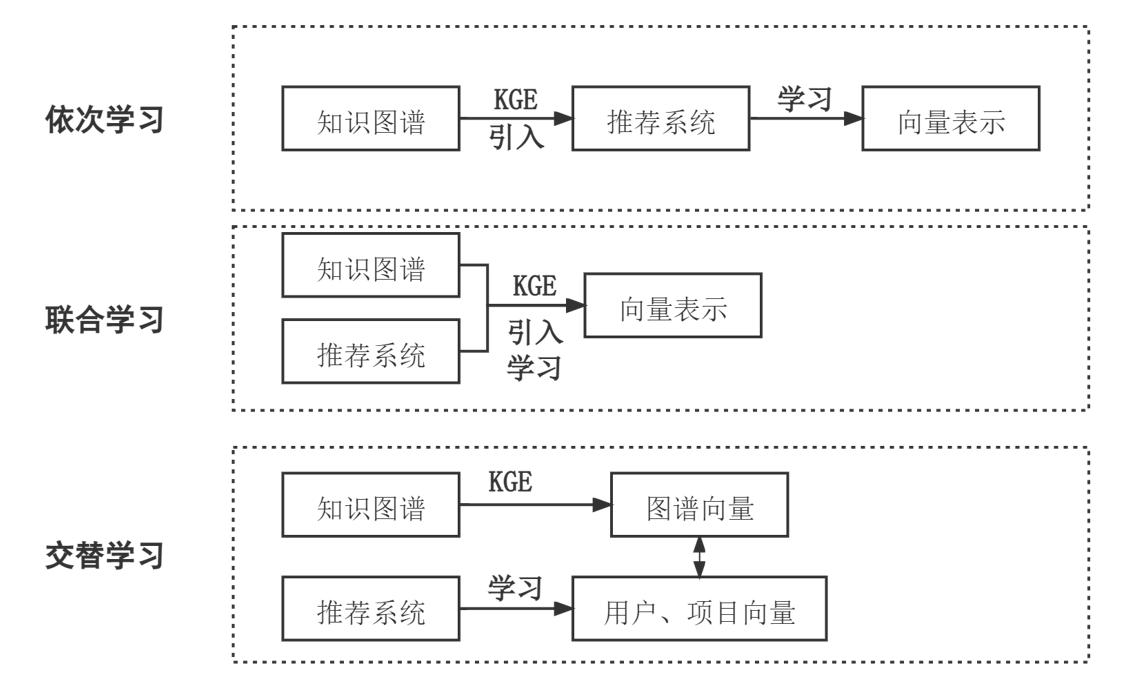
\includegraphics[width=10cm]{p2.png}% 图片相对位置
		\vspace{-0.5cm}
		\caption{基于知识图谱嵌入的推荐系统分类} % 图片标题 
	\end{figure}
	基于图嵌入的知识图谱推荐系统能够充分利用知识图谱语义关系,且受图谱扩展影响较小。在其发展过程中逐渐诞生了Node2Vec\upcite{8}、entity2rec\upcite{9}、DKN\upcite{10}、SI-MKR\upcite{11}等一系列模型。但是,该类模型在推荐中也损失了	图谱中的多跳关系利用,导致部分推荐结果缺乏可解释性。
	
	 \subsection{基于混合的推荐}
	虽然上述两种方法都利用知识图谱对推荐系统的应用进行了改进,但是对知识图谱充分利用存在一定局限性。因此基于混合的推荐逐渐被创建,其主要思想是:首先在整个图谱上通过传播的方式获取用户的偏好,然后通过图嵌入对用户偏好进行特征学习,再利用推荐模块实现推荐。
	
	基于混合的推荐包括三个经典模型:RippleNet\upcite{12}、KGCN\upcite{13}和KGAT\upcite{14}及其衍生系列。
	
	RippleNet模型2018年由Wang Hongwei 等\upcite{12}提出,该模型首先给定一个项
	目和一个用户,然后将项目经过嵌入转化的低维向量不断同用户周围的 n 跳项
	目转化向量进行交互计算,最后组成该用户的向量表示,再通过与给定项目转
	化向量计算获得用户点击概率从而完成推荐。计算公式如下:

	\begin{equation}
	\begin{array}{l}
	\hat{y}_{u v}=\sigma\left(u^{T} v\right)=\frac{1}{1+\exp \left(-u^{T} v\right)} \\
	u=o_{u}^{1}+o_{u}^{2}+\cdots+o_{u}^{H} \\
	o_{u}^{1}=\sum\left(h_{i}, r_{i}, t_{i}\right) \in S_{u}^{1} P_{i} t_{i} \\
	p_{i}=\operatorname{softmax}\left(v^{T} R_{i} h_{i}\right)=\frac{\exp \left(v^{T} R_{i} h_{i}\right)}{\left(\sum(h, r, t) \in S_{u}^{1} \exp \left(v^{T} R h\right)\right)}
	\end{array}
	\end{equation}
	
	\small{注:式中$\hat{y}_{uv}$表示用户$u$点击项目$v$的概率,$h_i$表示用户$u$的历史点击项目的1-hop邻居,$r_i$代表节点间关系,$t_i$代表$h_i$,$r_i$三元组中尾节点,v表示用户点击的商品,$R_i$是两者之间关系,$p_i$代表两者的归一化相似度。
	
	\normalsize
	虽然该模型通过混合的方法对于借助知识图谱实现的推荐取得了阶段性成果,但是同样存在忽视关系重要性、计算成本大和计算冗余的问题。
	
	KGCN模型\upcite{13}结合了知识图谱和图卷积神经网络。该模型首先需要设置节点多跳参数,将节点多跳范围内邻域作为感知野,然后将邻域节点在特定用户关系范围内的得
	分作为权重,并用加权结果表示邻域节点向量,进而完成项目向量表示。得到向量表示后同样利用用户向量与项目向量的内积搭配 sigmoid 函数计算点击概率
	完成推荐。
	
	KGAT\upcite{14}全称又叫“知识图谱注意力神经网络”,该模型在CKG嵌入层将用户—项目交互矩阵与知识图谱相结合,通过嵌入的方式得到图谱项目向量表示,然后在注意力嵌入传播层通过邻居的多跳节点递归传播向量实现项目表示增强,通过基于知识图谱的注意力机制计算关系权重,聚合信息后完成节点向量表示,
	最后在预测层通过向量计算并归一化得到用户点击概率并实现推荐。
	
	基于混合的推荐结合前面两种推荐思想的优势,既实现了对于知识图谱网络结构中连接关系的利用,又通过嵌入的思想实现实体和关系的低维空间向量表示,在表现出更优评分的同时,也为研究者带来了更大
	的资源消耗和更复杂的参数调优问题。如何解决该类模型导致的复杂问题,实
	现复杂模型下高效、精准、多样的推荐值得进一步探索。
	
	\section{总结}
	本文介绍了以协同过滤为代表的传统推荐系统,以及基于连接、基于嵌入、基于混合的推荐系统,并着重介绍了一些该领域经典和最新的模型。此外,文献\upcite{1}还介绍了更多相关领域的成果,具体内容如下表所示:
	

	\begin{table}[H]
		\centering
		\caption{基于知识图谱的推荐模型对比表}
		\begin{tabular}{cccc}
			\hline
			\multicolumn{2}{c}{推荐模型} & 年份 & 核心算法/思想 \\ \hline
			\multirow{9}{*}{基于连接的推荐} & HeteroMF & 2013 & 集体矩阵分解(CMF) \\
			& Hete-MF & 2013 & 矩阵分解(MF) \\
			& HeteRec-p & 2014 & 贝叶斯排序(BPR) \\
			& Hete-CF & 2014 & 协同过滤(CF) \\
			& SemRec & 2015 & 加权元路径相似性度量 \\
			& GraphLF & 2016 & 概率逻辑系统(ProPPR) \\
			& FMG & 2017 & 矩阵分解(MF) \\
			&  &  & 主成分分析(PCA) \\
			&  &  & 线性判别分析(LDA) \\ \hline
			\multirow{14}{*}{基于嵌入的推荐} & Node2Vec & 2016 & 随机梯度下降(SGD) \\
			&  &  & 离散傅立叶变换(DFT) \\
			&  &  & 广度优先抽样(BFS) \\
			& entity2rec & 2017 & node2vec \\
			&  &  & LambdaMart \\
			&  &  & Adarank \\
			& DKN & 2018 & 卷积神经网络(CNN) \\
			&  &  & 深度神经网络(DNN) \\
			&  &  & 注意力机制 \\
			& RKGE & 2018 & 循环神经网络(RNN) \\
			& MKR & 2019 & 多层感知器(MLP) \\
			&  &  & 多任务学习(MTL) \\
			& SI-MKR & 2020 & 多层感知器(MLP) \\
			&  &  & 卷积神经网络(CNN) \\ \hline
			\multirow{16}{*}{基于混合的推荐} & RippleNet & 2018 & 偏好传播 \\
			& KGCN & 2019 & 图卷积神经网络(GCN) \\
			&  &  & 注意力机制 \\
			& KGAT & 2019 & 图卷积神经网络(GCN) \\
			&  &  & TransR \\
			&  &  & 注意力机制 \\
			& RecKGC & 2019 & 知识图谱补全(KGC) \\
			&  &  & 注意力机制 \\
			& GraphRec & 2019 & 图神经网络(GNNs) \\
			&  &  & 多层感知器(MLP) \\
			& NIAGCN & 2020 & 逐层邻居聚合(PNA) \\
			&  &  & 并行图卷积网络 \\
			&  &  & 跨深度集成(CDE) \\
			& MBGCN & 2020 & 图卷积神经网络(GCN) \\
			& NeuACF & 2021 & 深度神经网络(DNN) \\
			&  &  & 自注意力机制 \\ \hline
		\end{tabular}
	\end{table}
	
\begin{thebibliography}{9}%宽度9
	\bibitem{1}  朱冬亮,文奕,万子琛.基于知识图谱的推荐系统研究综述[J/OL].数据分析与知识发现:1-16[2021-12-08].http://kns.cnki.net/kcms/detail/10.1478.G2.20211020.1438.004.html.
	\bibitem{2} 袁泉,成振华,江洋.基于知识图谱和协同过滤的电影推荐算法研究[J].计算机工程与科学,2020,42(04):714-721.
	\bibitem{3}
	HANSEN C, HANSEN C, MAYSTRE L, et al. Contextual and Sequential User Embeddings for Large-Scale
	Music Recommendation[C]. In: Fourteenth ACM Conference on Recommender Systems,NewYork,USA: ACM,
	2020: 53-62
	\bibitem{4}
	LUO C, PANG W, WANG Z, et al. Hete-CF: Social-Based Collaborative Filtering Recommendation Using
	Heterogeneous Relations[C]. In: Proceedings of the 2014 IEEE International Conference on Data Mining, Beijing,
	China:IEEE,2014:14-17.
	\bibitem{5}
	ZHAO H, YAO Q, LI J, et al. Meta-Graph Based Recommendation Fusion over Heterogeneous Information
	Networks[C]. In: Proceedings of the 23rd ACM SIGKDD International Conference on Knowledge Discovery and
	Data Mining, Halifax, NS, Canada: Association for Computing Machinery,2017: 635–644.
	\bibitem{6}		
	CATHERINE R, COHEN W. Personalized Recommendations using Knowledge Graphs: A Probabilistic Logic
	Programming Approach[C]. In: Proceedings of the 10th ACM Conference on Recommender Systems,Boston,
	Massachusetts, USA; Association for Computing Machinery. 2016: 325–332.	
	\bibitem{7}	
	王 鸿 伟. 如 何 将 知 识 图 谱 特 征 学 习 应 用 到 推 荐 系 统 ? [EB/OL]. [2021-06-08].
	https://www.jiqizhixin.com/articles/2018-06-06-5.(Wang Hongwei. How to Apply Knowledge Graph Feature
	Learning to Recommendation System? [EB/OL]. [2021-06-08]. https://www.jiqizhixin.com/articles/2018-06-06-5.)
	
	\bibitem{8}	
	GROVER A, LESKOVEC J. node2vec: Scalable Feature Learning for Networks[C]. In: Proceedings of the
	22nd ACM SIGKDD International Conference on Knowledge Discovery and Data Mining,San Francisco, California,
	USA:Association for Computing Machinery,2016: 855–864.
	\bibitem{9}	
	PALUMBO E, RIZZO G, TRONCY R. entity2rec: Learning User-Item Relatedness from Knowledge Graphs
	for Top-N Item Recommendation[C]. In :Proceedings of the Eleventh ACM Conference on Recommender Systems,
	Como, Italy:Association for Computing Machinery, 2017: 32–36.
	\bibitem{10}	
	WANG H, ZHANG F, XIE X, et al. DKN: Deep Knowledge-Aware Network for News Recommendation[C].
	In :Proceedings of the 2018 World Wide Web Conference, Lyon, France: International World Wide Web Conferences
	Steering Committee, 2018: 1835–1844.
	\bibitem{11}	
	WANG Y Q, DONG L Y, ZHANG H, et al. An Enhanced Multi-Modal Recommendation Based on Alternate
	Training With Knowledge Graph Representation[J]. Ieee Access, 2020, 8(213012-213026).
	\bibitem{12}	
	WANG H, ZHANG F, WANG J, et al. RippleNet: Propagating User Preferences on the Knowledge Graph for
	Recommender Systems[C]. In: Proceedings of the 27th ACM International Conference on Information and
	Knowledge Management,Torino, Italy:Association for Computing Machinery,2018: 417–426.
	\bibitem{13}	
	WANG H, ZHAO M, XIE X, et al. Knowledge Graph Convolutional Networks for Recommender Systems
	[C]. In: The World Wide Web Conference. San Francisco, CA, USA: Association for Computing Machinery, 2019.
	3307–3313
	\bibitem{14}	
	WANG X, HE X, CAO Y, et al. KGAT: Knowledge Graph Attention Network for Recommendation[C]. In:
	Proceedings of the 25th ACM SIGKDD International Conference on Knowledge Discovery \&amp; Data Mining,
	Anchorage, AK, USA; Association for Computing Machinery, 2019: 950–958
									
\end{thebibliography}	


\end{document} 



